\section{Experiments}\label{sec:experiments}
We evaluate the proposed algorithms on the following scenario: a collection of 3d-points $P = \{ p_1,\dots,p_s \} \subseteq \R^3$ is sampled from a number of $t$ planes which contain the coordinate origin. We wish to partition the resulting point cloud in such a way that makes the underlying set of planes obvious: i.e., all points that were sampled from a given plane are part of the same partition, distinct from the partitions of the other planes. Figure \ref{fig:point_cloud_examples} shows some examples on possible partitions. The points are generated as follows:
\begin{enumerate}
    \item Every plane is defined by a normal vector and an orientation, i.e. we have vectors $\vec{n}_1,\dots,\vec{n}_t \in \R^3$ and orientations $\vec{o}_1,\dots,\vec{o}_t \in \R^3$. For each plane, we draw $\lambda_i,\lambda_i'$ from $\mathcal{U}([-\pi,\pi))$, and $x_i,x_i'$ from $\mathcal{U}([0,1))$ and determine $\varphi_i = \arccos(2x_i-1), \varphi_i' = \arccos(2x_i'-1)$\footnote{Source: Jason Davies, \href{https://www.jasondavies.com/maps/random-points/}{https://www.jasondavies.com/maps/random-points/}. Accessed on December 6th, 2020.}. The vectors are computed by $$ \vec{n}_i = \begin{bmatrix} \sin(\varphi_i) \cos(\lambda_i) \\ \sin(\varphi_i)\sin(\lambda_i) \\ \cos(\varphi_i) \end{bmatrix},\quad \vec{o}_i = \mathrm{norm} \left( \begin{bmatrix} \sin(\varphi_i') \cos(\lambda_i') \\ \sin(\varphi_i')\sin(\lambda_i') \\ \cos(\varphi_i') \end{bmatrix} \times \vec{n}_i \right), $$ where $\mathrm{norm}(\vec{h})=\frac{1}{||\vec{h}||} \vec{h} $ ($\vec{n}_i$ is already normalized, since it describes a point on the unit-sphere).
    \item For every point $p_i$, three components are sampled: the 2d-position on the plane $x_i,y_i$ from $\mathcal{U}([-1,1])$, and a noise-component $z_i$ from $\mathcal{U}([-\epsilon,\epsilon])$ (where $\epsilon$ indicates the level of noise). The point is then transformed into plane-space, i.e. $$ p_i = x_i \vec{o}_i + y_i \mathrm{norm}(\vec{o}_i \times \vec{n}_i) + z_i \vec{n}_i$$
\end{enumerate}
For three points $u,v,w \in P$, we define the following cost-structure
\begin{align*}
    c(\{u,v,w\}) = 0,\quad c'(\{u,v,w\}) = \mathrm{d}(\{ u,v,w \},(0,0,0)) - \tau,
\end{align*}
where $\mathrm{d}(\{u,v,w\},p)$ is the distance between the plane that contains $u,v$ and $w$ and $p$ (``$\cdot$'' is the dot-product in this case):
\begin{align*}
    \mathrm{d}(\{u,v,w\},p) = \frac{\vec{n} \cdot (u - p)}{||\vec{n}||},\quad \vec{n} = (v-u)\times (w-u),
\end{align*}
and $\tau$ is some small value. Therefore, if the distance from the plane spanning over $u,v$ and $w$ to the origin ist smaller than $\tau$, it is considered ``good'' when $u,v$ and $w$ are part of the same partition and if the distance is large, it is considered ``bad''.

\begin{figure}
    \centering
    \begin{subfigure}{.45\textwidth}
        \centering
        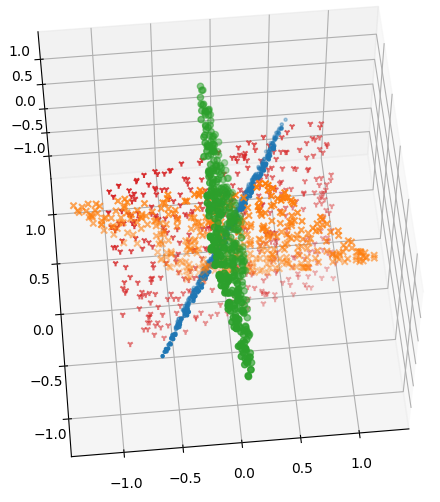
\includegraphics[width=\textwidth]{pics/points-400-400-400-400.png}
        \caption{Point cloud consisting of four planes with 400 points each and noise $\epsilon=0.01$.}
    \end{subfigure}%
    \hspace{2em}
    \begin{subfigure}{.45\textwidth}
        \centering
        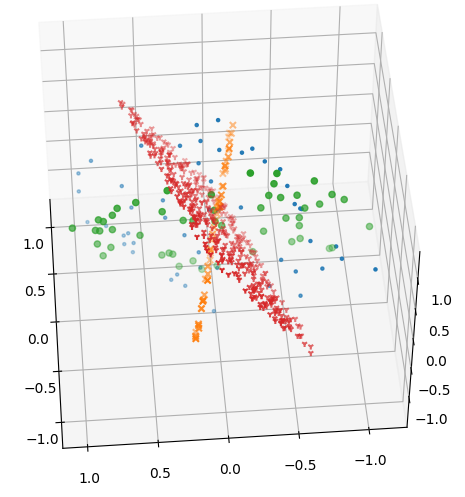
\includegraphics[width=\textwidth]{pics/points-50-50-50-400.png}
        \caption{Point cloud consisting of four planes, of which three have 50 points and one has 400 points with noise $\epsilon=0.01$.}
    \end{subfigure}
    \caption{Two possible point clouds.} \label{fig:point_cloud_examples}
\end{figure}

\begin{table}
    \centering
    \begin{tabular}{l|l}
        dataset & planes $\times$ number \\
        \hline
        0 & $3 \times 30  $ \\
        1 & $3 \times 80  $ \\
        2 & $3 \times 150 $ \\
        3 & $4 \times 250 $ \\
        4 & $5 \times 300 $
    \end{tabular}
    \caption{Generated datasets and executed runs. Every set contains a number of planes with an equal amount of points. Noise level is $\epsilon = 0.01$.}
\end{table}

\begin{table}
    \begin{tabular}{lllll|ll}
        run & dataset & {\bf ip} & $N$ & $M$ & {\bf or} [s] & {\bf iter} \\
        \hline 
        0-S-S  & 0 & 1 & 40 &  1000       & 3.00 & 153      \\    
        0-E-S  & 0 & 1 & -- &  1000       & 37.57 & 109     \\    
        0-S-E  & 0 & 1 & 40 &  --         & 4.73 & 148      \\    
        0-E-E  & 0 & 1 & -- &  --         & 23.80 & 100     \\   
        \hline 
        1-S-S  & 1 & 1 & 40 &  5000       & 18.31 & 518     \\    
        1-E-S  & 1 & 1 & -- &  5000       & 1348.06 & 511   \\    
        1-S-E  & 1 & 1 & 40 &  --         & 62.00 & 439     \\    
        1-E-E  & 1 & 1 & -- &  --         & 511.49 & 131    \\    
        \hline
        2-S-S  & 2 & 1 & 50 &  5000       & 43.98 & 958     \\    
        3-S-S  & 3 & 1 & 50 & 10000       & 322.22 & 4607   \\    
        4-S-S  & 4 & 1 & 50 & 15000       & 1280.99 & 10694 \\    
        \hline
        2-S-SL & 2 & 1 & 50 &   500       & 37.80 & 1769    \\    
        2-SL-S & 2 & 1 &  5 &  5000       & 78.19 & 10480   \\    
        \hline
        2-S-S-IP10  & 2 &  10 & 50 & 5000 & 62.54 & 1309    \\
        2-S-S-IP50  & 2 &  50 & 50 & 5000 & 74.12 & 1582    \\
        2-S-S-IP100 & 2 & 100 & 50 & 5000 & 88.77 & 1937    \\
    \end{tabular}
    \caption{Every run with the corresponding dataset it was executed on, the number of {\bf i}nitial {\bf p}artitions, the number of neighbours $N$ and samples $M$ that are selected per iteration, the {\bf o}verall {\bf r}untime and number of {\bf iter}ations. If entries for $N$ or $M$ are ``--'', then this means that the complete neighbourhood was considered, or the reduced costs where computed explicitly. For each run, $\tau = 0.1$ was selected.} \label{tab:data}
\end{table}

The algorithms are evaluated in the four following settings. First, the deterministic greedy search is compared with randomized versions, in which only a certain subset of neighbours is selected and/or the reduced cost is only approximated. This is done on the two datasets 0 and 1, in which dataset 0 contains $3 \times 30$ points, and dataset 1 overall $3 \times 80$ points. In the second setting, problems with larger input-sizes are considered and solved by the randomized greedy search algorithm (dataset 2,3 and 4 with $3 \times 150$, $4 \times 250$ and $5 \times 300$ points respectively). The penultimate setting examines the impact of low neighbourhood- and sampling sizes regarding the cost function. Finally, the randomized greedy search algorithm is initialized with multiple randomly assigned partitions. The results are shown in figures \ref{fig:setting11}, \ref{fig:setting12}, \ref{fig:setting2}, \ref{fig:setting3} and \ref{fig:setting4}. The upper rows show how much the costs are reduced in each iteration, the middle rows contain the used time per iteration -- the cumulative time to compute the reduced cost for each neighbour in orange, and the time required to compute the neighbourhood in blue -- and the last rows show the number of partitions per iteration.

\paragraph{Setting 1.} The results are depicted in figures \ref{fig:setting11} and \ref{fig:setting12}. When the complete neighbourhood is considered, as for run 0-E-S, 0-E-E, 1-E-S and 1-E-E, the used time per iteration is clearly dependent on the number of partitions. This is obvious from analysis of algorithm \ref{alg:moveenum}, since the number of neighbours grows in size $O(|V| \cdot \Pi(\idx))$. Considering the complete neighbourhood has probably the largest impact on the overall runtime, as can be seen in table \ref{tab:data}. 


\begin{landscape}
    \begin{figure}
        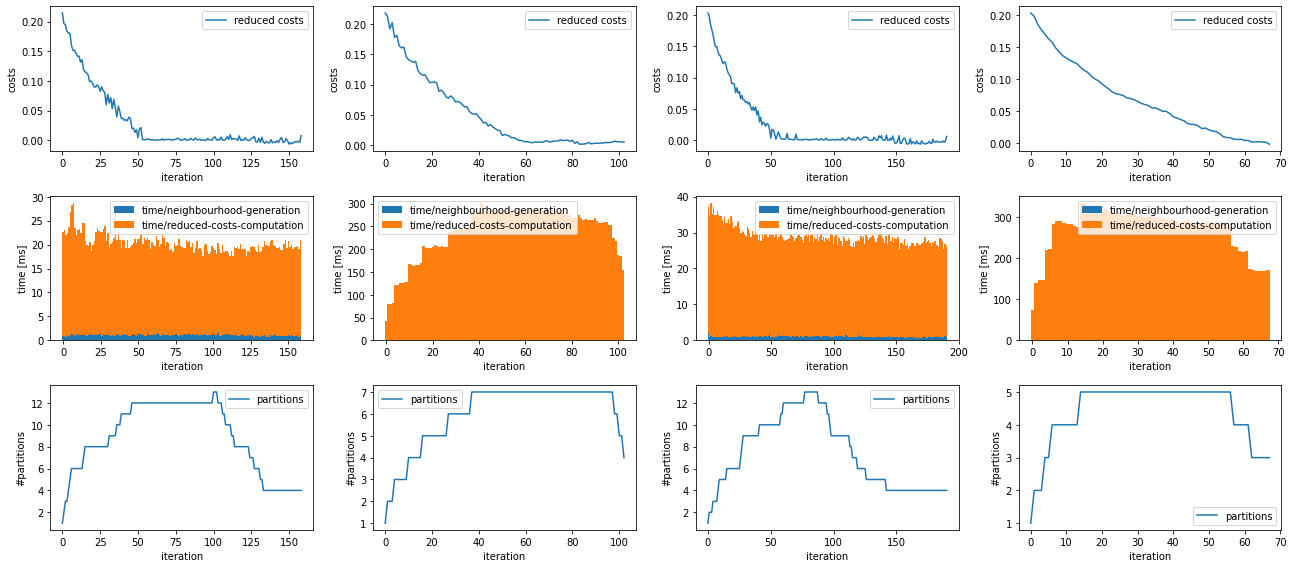
\includegraphics[width=25cm]{pics/experiments_0.png}
        \caption{From left to right: run 0-S-S, 0-E-S, 0-S-E, 0-E-E.}
        \label{fig:setting11}
    \end{figure}
\end{landscape}


\begin{landscape}
    \begin{figure}
        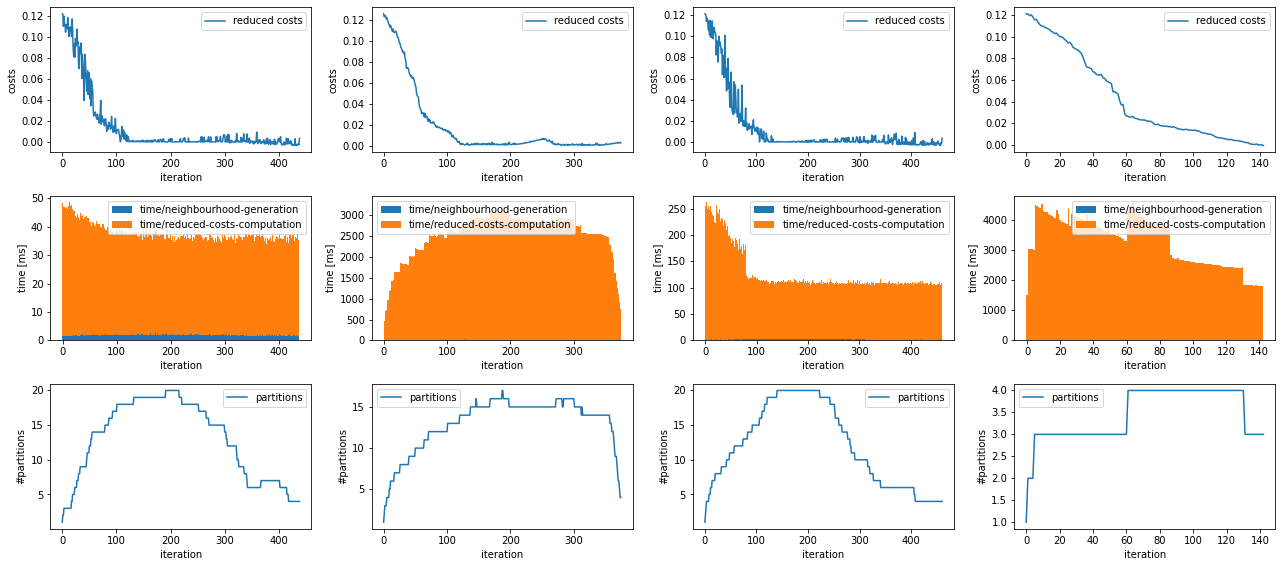
\includegraphics[width=25cm]{pics/experiments_1.png}
        \caption{From left to right: run 1-S-S, 1-E-S, 1-S-E, 1-E-E.}
        \label{fig:setting12}
    \end{figure}
\end{landscape}

\begin{landscape}
    \begin{figure}
        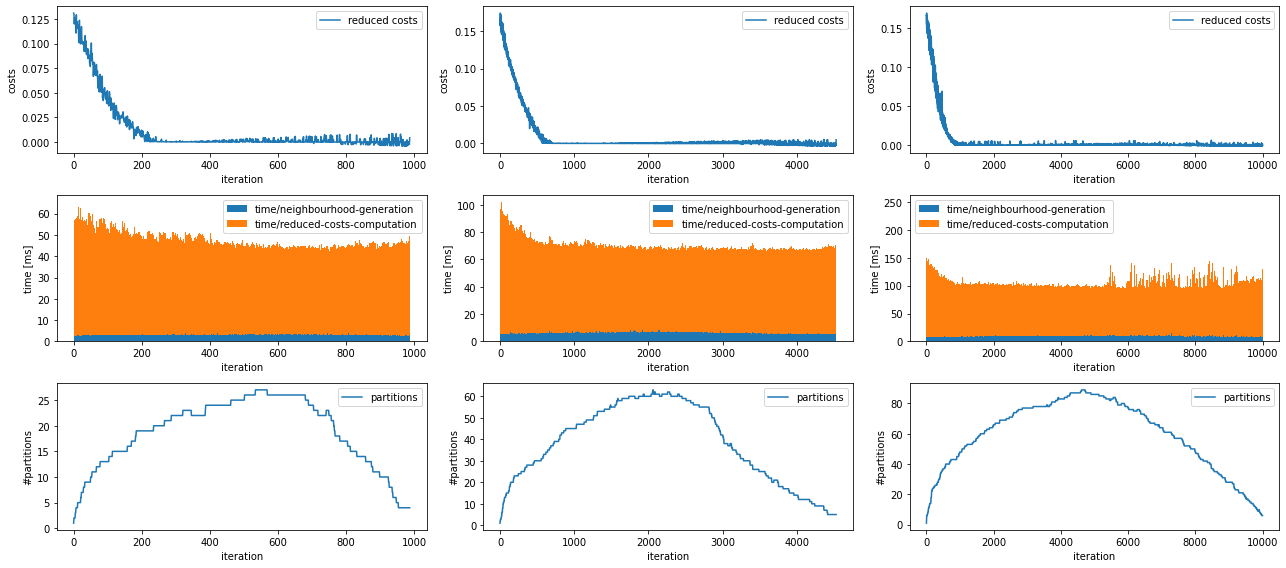
\includegraphics[width=25cm]{pics/experiments_2.png}
        \caption{From left to right: run 2-S-S, 3-S-S, 4-S-S.}
        \label{fig:setting2}
    \end{figure}
\end{landscape}

\begin{landscape}
    \begin{figure}
        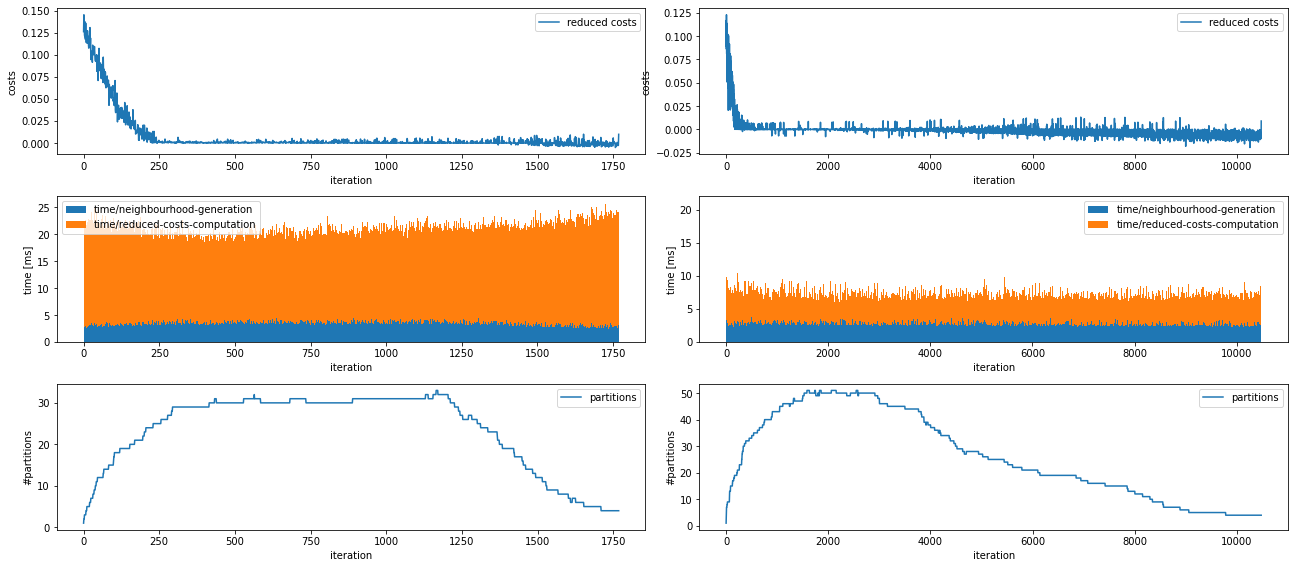
\includegraphics[width=25cm]{pics/experiments_3.png}
        \caption{From left to right: run 2-S-SL, 2-SL-S.}
        \label{fig:setting3}
    \end{figure}
\end{landscape}

\begin{landscape}
    \begin{figure}
        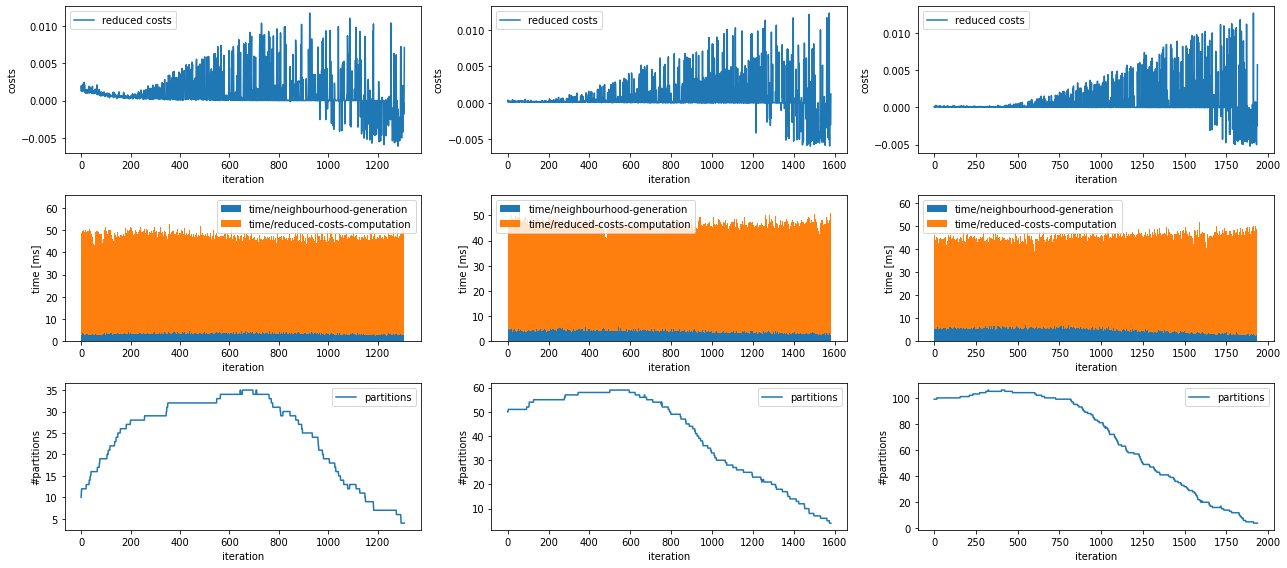
\includegraphics[width=25cm]{pics/experiments_4.png}
        \caption{From left to right: run 2-S-S-IP10, 2-S-S-IP50, 2-S-S-IP100.}
        \label{fig:setting4}
    \end{figure}
\end{landscape}


% points i want to make:
% sampling neighbours and costs is really efficient when |V| grows larger
% evaluating the neighbourhood and computing the complete costs does not really work for large |V|
% M needs to be choosen sufficiently large, or else it does not converge
% possible improvements: sample only vertices such that the resulting costs is non-zero
% M needs to be somewhat proportional to |V| and the expected variance: i.e., dependent on the 
% number of partitions
% number of planes -> impact on the variance
% do we need 